
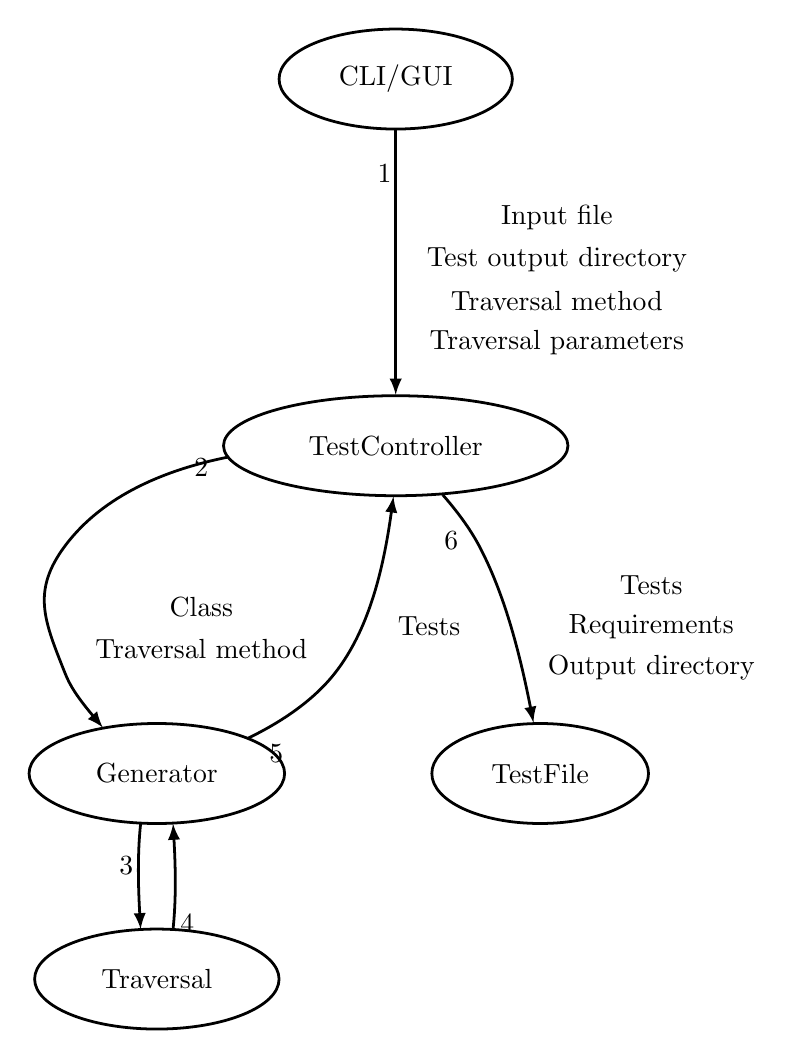
\begin{tikzpicture}[>=latex,line join=bevel,]
  \pgfsetlinewidth{1bp}
%%
\pgfsetcolor{black}
  % Edge: Generator -> TestController
  \draw [->] (78.932bp,104.75bp) .. controls (90.216bp,110.24bp) and (102bp,117.86bp)  .. (110bp,128bp) .. controls (121.99bp,143.21bp) and (127.46bp,164.45bp)  .. (131.19bp,191.75bp);
  \definecolor{strokecol}{rgb}{0.0,0.0,0.0};
  \pgfsetstrokecolor{strokecol}
  \draw (144bp,145bp) node {Tests};
  \draw (89bp,99bp) node {5};
  % Edge: CLI/GUI -> TestController
  \draw [->] (132bp,323.74bp) .. controls (132bp,301.98bp) and (132bp,264.32bp)  .. (132bp,228.33bp);
  \draw (190bp,292bp) node {Input file};
  \draw (190bp,277bp) node {Test output directory};
  \draw (190bp,262bp) node {Traversal method};
  \draw (190bp,247bp) node {Traversal parameters};
  \draw (128bp,308bp) node {1};
  % Edge: Traversal -> Generator
  \draw [->] (51.827bp,35.941bp) .. controls (52.718bp,44.261bp) and (52.964bp,54.49bp)  .. (51.84bp,73.937bp);
  \draw (57bp,38bp) node {4};
  % Edge: TestController -> Generator
  \draw [->] (72.018bp,205.98bp) .. controls (49.858bp,201.59bp) and (26.805bp,192.45bp)  .. (13bp,174bp) .. controls (0.7518bp,157.63bp) and (5.4548bp,147bp)  .. (13bp,128bp) .. controls (14.675bp,123.78bp) and (17.126bp,119.78bp)  .. (26.561bp,108.54bp);
  \draw (62bp,152bp) node {Class};
  \draw (62bp,137bp) node {Traversal method};
  \draw (62bp,202bp) node {2};
  % Edge: TestController -> TestFile
  \draw [->] (148.92bp,192.32bp) .. controls (153.71bp,186.86bp) and (158.55bp,180.51bp)  .. (162bp,174bp) .. controls (170.89bp,157.2bp) and (176.44bp,136.5bp)  .. (181.59bp,110.26bp);
  \draw (224bp,160bp) node {Tests};
  \draw (224bp,145bp) node {Requirements};
  \draw (224bp,130bp) node {Output directory};
  \draw (152bp,176bp) node {6};
  % Edge: Generator -> Traversal
  \draw [->] (40.16bp,73.937bp) .. controls (39.275bp,65.598bp) and (39.036bp,55.364bp)  .. (40.173bp,35.941bp);
  \draw (35bp,59bp) node {3};
  % Node: CLI/GUI
\begin{scope}
  \definecolor{strokecol}{rgb}{0.0,0.0,0.0};
  \pgfsetstrokecolor{strokecol}
  \draw (132bp,342bp) ellipse (42bp and 18bp);
  \draw (132bp,342bp) node {CLI/GUI};
\end{scope}
  % Node: TestController
\begin{scope}
  \definecolor{strokecol}{rgb}{0.0,0.0,0.0};
  \pgfsetstrokecolor{strokecol}
  \draw (132bp,210bp) ellipse (62bp and 18bp);
  \draw (132bp,210bp) node {TestController};
\end{scope}
  % Node: TestFile
\begin{scope}
  \definecolor{strokecol}{rgb}{0.0,0.0,0.0};
  \pgfsetstrokecolor{strokecol}
  \draw (184bp,92bp) ellipse (39bp and 18bp);
  \draw (184bp,92bp) node {TestFile};
\end{scope}
  % Node: Generator
\begin{scope}
  \definecolor{strokecol}{rgb}{0.0,0.0,0.0};
  \pgfsetstrokecolor{strokecol}
  \draw (46bp,92bp) ellipse (46bp and 18bp);
  \draw (46bp,92bp) node {Generator};
\end{scope}
  % Node: Traversal
\begin{scope}
  \definecolor{strokecol}{rgb}{0.0,0.0,0.0};
  \pgfsetstrokecolor{strokecol}
  \draw (46bp,18bp) ellipse (44bp and 18bp);
  \draw (46bp,18bp) node {Traversal};
\end{scope}
%
\end{tikzpicture}

